%% !TEX root = ../../main.tex
\documentclass[crop=true]{standalone}

\usepackage{tikz}
\usetikzlibrary{calc,positioning,decorations.text,backgrounds}
\usepackage{etoolbox}
\usepackage{standalone}

\begin{document}
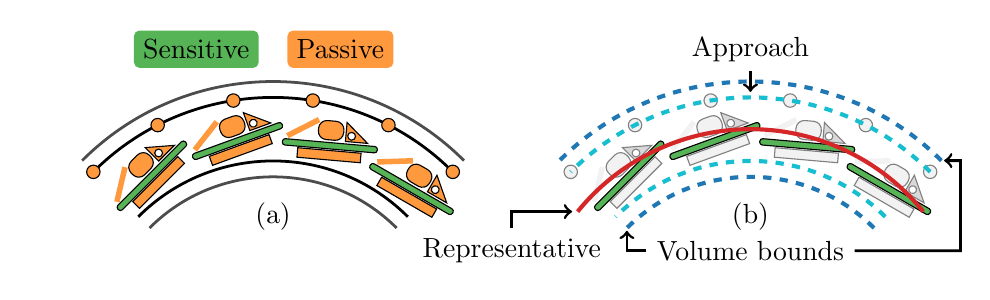
\begin{tikzpicture}[scale=1.0]

    \definecolor{tab1}{RGB}{31,119,180}
    \definecolor{tab2}{RGB}{255,127,14}
    \definecolor{tab3}{RGB}{44,160,44}
    \definecolor{tab4}{RGB}{214,39,40}
    \definecolor{tab5}{RGB}{148,103,189}
    \definecolor{tab6}{RGB}{140,86,75}
    \definecolor{tab7}{RGB}{227,119,194}
    \definecolor{tab8}{RGB}{127,127,127}
    \definecolor{tab9}{RGB}{188,189,34}
    \definecolor{tab10}{RGB}{23,190,207}

    \def\passivec{tab2!80}
    \def\sensitivec{tab3!80}

    \def\ao{90}
    \def\as{45}
    \pgfmathsetmacro{\al}{-\as+\ao}
    \pgfmathsetmacro{\ar}{\as+\ao}
    \def\ri{6}
    \def\ro{8}
    \def\rvi{5.5}
    \def\rvo{8.5}
    \pgfmathsetmacro{\rm}{(\ro+\ri)/2}
    
    \newcommand{\dbox}[4]{
      \def\w{#2}
      \def\h{#3}
      \node[#4,inner sep=0,minimum width=\w,minimum height=\h] (#1) at (0,0) {};
    }
    \def\n{5}

    % \coordinate (gtr) at ({\linewidth},3cm);
    % \fill[red] (0,0) circle(3pt);
    % \coordinate (gright) at ({0.99\linewidth},0);
    \coordinate (gright) at ({\linewidth-2mm},0);
    \coordinate (gleft) at (0,0);


    \pgfmathsetmacro{\wcalc}{2*cos(\al)*\rvo * 1cm}
    \pgfmathsetmacro{\wscale}{0.4 / (\wcalc/\linewidth)}
    \def\gs{\wscale}

    \coordinate (gmid) at ({0.5*\linewidth},{\gs*\rm});

    % \fill[red] (gmid) circle(3pt);
    
    % \node at (0,-3) {\wcalc - \wscale};
    % \draw[red,line width=1pt,->] (0,0) -- (\linewidth, 0);

    \begin{scope}[shift={({0.25*\linewidth},0)}]
      \begin{scope}[scale=\gs]
      %   \coordinate (bl) at ({-cos(\al)*\ro}, {sin(\al)*\ri});
        \coordinate (bl) at ({-cos(\al)*\rvo}, {sin(\al)*\rvi});
        \coordinate (tr) at ({cos(\al)*\rvo}, \rvo);
        \coordinate (pad) at (6pt,6pt);
        \clip ($(bl-|gleft) - (pad)$) rectangle ($(tr) + (pad)$);
      
        \node at (0,{sin(\al)*\ri}) {(a)};
      
        \foreach \r in {\ri,\ro} {
          \draw[line width=1pt] (0,0) ++ (\al:\r) arc (\al:\ar:\r);
        }
        
        \foreach \r in {\rvi,\rvo} {
          \draw[line width=1pt,black!70] (0,0) ++ (\al:\r) arc (\al:\ar:\r);
        }
      
        \foreach \i in {0,...,\n} {
          \pgfmathsetmacro{\a}{\al + (\ar-\al)/\n * \i}
          \draw[fill=\passivec] (\a:\ro) circle(6pt);
        }
      
      
        \foreach \i in {0,...,3} {
          \pgfmathsetmacro{\ma}{-\as + \i*25 + 5}
          \begin{scope}[rotate=\ma,transform shape]
            \begin{scope}[transform shape,shift={(0,\rm)},rotate=10]
              \begin{scope}[shift={(0,0.2)}]
                \dbox{b1}{8mm}{6mm}{draw,fill=\passivec,rounded corners=3pt}
              \end{scope}
              \begin{scope}[shift={($(b1.south) + (0,-2pt)$)}]
                \dbox{b2}{3cm}{2mm}{draw,anchor=north,fill=\sensitivec,rounded corners=1pt}
              \end{scope}
              \begin{scope}[shift={($(b2.south) + (0,-1pt)$)}]
                \dbox{b3}{2cm}{3mm}{draw,anchor=north,fill=\passivec}
              \end{scope}
      
              \begin{scope}[shift={($(b1.south east) + (2pt,0pt)$)}]
                \draw[fill=\passivec] (0,0) --(7mm,0) --(0,6mm) -- cycle;
                \draw[fill=white] (1.8mm,1.8mm) circle(3.5pt);
              \end{scope}
              \draw[line width=2pt,shorten >=2pt,\passivec] (b1.north west) -- (b2.north west);
            \end{scope}
          \end{scope}
        }
      
      \end{scope}
    \end{scope}
    
    \def\thec{black!5}

    
    \begin{scope}[shift={({0.75\linewidth},0)}]
      \begin{scope}[draw=black!50,scale=\gs]
        \coordinate (bl) at ({-cos(\al)*\rvo}, {sin(\al)*\rvi});
        \coordinate (tr) at ({cos(\al)*\rvo}, \rvo);
        \coordinate (pad) at (6pt,6pt);
        \clip ($(bl) - (pad)$) rectangle ($(tr) + (pad)$);
      
        \node at (0,{sin(\al)*\ri}) {(b)};
      
        \foreach \i in {0,...,\n} {
          \pgfmathsetmacro{\a}{\al + (\ar-\al)/\n * \i}
          \draw[fill=\thec] (\a:\ro) circle(6pt);
        }
        
        \foreach \r in {\ri,\ro} {
          \draw[line width=1.5pt,tab10,dashed] (0,0) ++ (\al:\r) arc (\al:\ar:\r);
        }
        
        \foreach \r[count=\ri] in {\rvi,\rvo} {
          \draw[line width=1.5pt,tab1,dashed] (0,0) ++ (\al:\r) arc (\al:\ar:\r) coordinate[at end] (vl\ri) coordinate[at start] (vr\ri);
        }
      
        \coordinate (appo) at (90:\ro);
      
        \foreach \i in {0,...,3} {
          \pgfmathsetmacro{\ma}{-\as + \i*25 + 5}
          \begin{scope}[rotate=\ma,transform shape]
            \begin{scope}[transform shape,shift={(0,\rm)},rotate=10]
              \begin{scope}[shift={(0,0.2)}]
                \dbox{b1}{8mm}{6mm}{draw,fill=\thec,rounded corners=3pt}
              \end{scope}
              \begin{scope}[shift={($(b1.south) + (0,-2pt)$)}]
                \dbox{b2}{3cm}{2mm}{draw,anchor=north,fill=\sensitivec,draw=black,rounded corners=1pt}
                \coordinate (sepo\i) at (15mm,0);
              \end{scope}
              \begin{scope}[shift={($(b2.south) + (0,-1pt)$)}]
                \dbox{b3}{2cm}{3mm}{draw,anchor=north,fill=\thec}
              \end{scope}
      
              \begin{scope}[shift={($(b1.south east) + (2pt,0pt)$)}]
                \draw[fill=black!15] (0,0) --(7mm,0) --(0,6mm) -- cycle;
                \draw[fill=white] (1.8mm,1.8mm) circle(3.5pt);
              \end{scope}
              \draw[line width=2pt,shorten >=2pt,\thec] (b1.north west) -- (b2.north west);
            \end{scope}
          \end{scope}
        }
        
        \def\aext{6}
        \draw[line width=1.5pt,tab4] (0,0) ++ ({\al-\aext}:\rm) arc ({\al-\aext}:{\ar+\aext}:\rm) coordinate[at end] (repo);
      
        \coordinate (label) at (0,{\rvo + 0.8});
        \coordinate (vlabloc) at (0,{\rvi - 0.8});
        \coordinate (bl2) at ({\ar}:\rvi);
      
      \end{scope}
    \end{scope}
    
    \node[anchor=base] (alabel) at (label) {Approach};
    % \node (vlab) at (vlabloc) {Volume bounds};
    % \node (slab) at ($(sepo0)-(0,2cm)$) {Sensitive};


    \begin{scope}[line width=1pt,shorten >=2pt]

      % \fill[red] (bl2-|gmid) circle(3pt);
      \node[below] (rlab) at (bl2-|gmid) {Representative};
      \draw[->] (rlab) |- (repo);

      \node (vlab) at (rlab-|{\linewidth*0.75},0) {Volume bounds};

      \draw[->,line width=1pt,shorten >=1pt] (vlab) -| (vl1);
      \coordinate (lix) at ($(vr2)!0.6!(vr2-|gright)$);
      \draw[->,line width=1pt,shorten >=1pt] 
        (vlab) 
        -- (vlab-|vr2) 
        node[below,pos=0.6] (xx) {}
        -| (lix) 
        -- (vr2);

      \draw[->] (alabel) -- (appo);

    %   \node[anchor=north east] (slabel) at ($(sepo0|-xx)-(3mm,0)$) {Sensitive};

    %   \draw[->] (slabel.east) -| (sepo0);
    
      \coordinate (ml) at (0, {(\ro + sin(\al)*\ri)/2});
      

    \end{scope}

    \begin{scope}[rounded corners=2pt]
      \node[fill=\sensitivec,left=5pt] at (alabel-|{0.25*\linewidth},0) {Sensitive};
      \node[fill=\passivec,right=5pt] at (alabel-|{0.25*\linewidth},0) {Passive};
    \end{scope}
    
\end{tikzpicture}
\end{document}